\section{La programmation orientée Objet}
\begin{frame}
	\begin{center}
	\huge
	La programmation Orientée Objet
	\end{center}
\end{frame}

\subsection{Notion d'objet} %%%%%%%%%%%%%%%%%%%%%%%%%%%%%%%%%%%%%%%%%
\begin{frame}
	\frametitle{Comme une boite}
	\begin{center}
	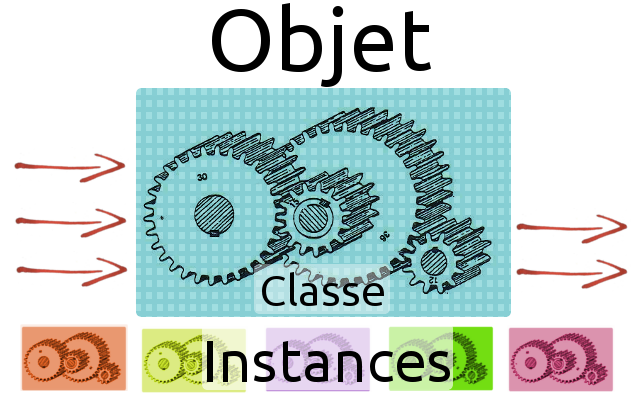
\includegraphics[width=9cm]{pics/explObj1.png}
	\end{center}
\end{frame}
\begin{frame}
	\frametitle{Attributs/Méthodes}
	\begin{center}
	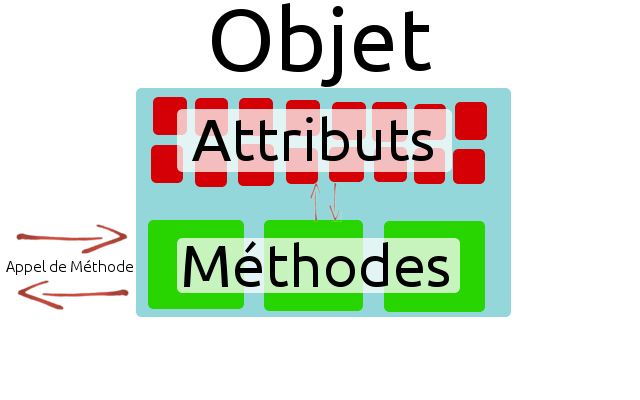
\includegraphics[width=9cm]{pics/explObj2.png}
	\end{center}
\end{frame}

\subsection{La déclaration d'un objet} %%%%%%%%%%%%%%%%%%%%%%%%%%%%%%
\begin{frame}
	\frametitle{Syntaxe}
	
\end{frame}

\begin{frame}
	\frametitle{Déclaration d'attribut}
	\framesubtitle{Simple}
	
\end{frame}

\begin{frame}
	\frametitle{Déclaration d'attribut}
	\framesubtitle{Modifiable}
	
\end{frame}

\begin{frame}
	\frametitle{Déclaration d'attribut}
	\framesubtitle{Lorsque rien ne va : Le type Option}
	
\end{frame}

\begin{frame}
	\frametitle{Déclaration de méthode}
	\framesubtitle{simple}
	
\end{frame}

\begin{frame}
	\frametitle{Déclaration de méthode}
	\framesubtitle{privée}
	
\end{frame}


\subsection{L'heritage} %%%%%%%%%%%%%%%%%%%%%%%%%%%%%%%%%%%%%%%%%%%%%
\begin{frame}

\end{frame}

\subsection{Le polymorphisme d'inclusion} %%%%%%%%%%%%%%%%%%%%%%%%%%%
\begin{frame}

\end{frame}
